\chapter{\textbf{Kiểm tra tất cả chức năng của hệ thống}}

\textbf{Tên hệ thống:} Hệ thống quản lý và phân phối máy in tập trung \\
\textbf{Domain:} ABC.local \\
\textbf{Server:} SRV-PRINT (192.168.244.10)

\section{Cấu hình môi trường kiểm tra}

\subsection{Cấu hình Server}
\begin{itemize}
    \item \textbf{Hostname:} SRV-PRINT
    \item \textbf{IP Address:} 192.168.244.10/24
    \item \textbf{Vai trò:} Domain Controller, DNS Server, Print Server
    \item \textbf{HĐH:} Windows Server 2016/2019/2022
\end{itemize}

\subsection{Cấu hình Client}
\begin{table}[htbp]
\centering\small
\begin{tabular}{|l|l|l|l|l|}
\hline
\textbf{Client} & \textbf{IP} & \textbf{Vai trò} & \textbf{User Domain} & \textbf{Máy in} \\ \hline
CL-Design & DHCP & In màu & user\_design & PRN\_Design\_01 \\ \hline
CL-Office & DHCP & In trắng đen & user\_office & PRN\_Office\_01 \\ \hline
CL-Accounting & DHCP & In B/W, audit & user\_accounting & PRN\_Accounting\_01 \\ \hline
\end{tabular}
\caption{Cấu hình các máy Client}
\end{table}

\noindent\textbf{Lưu ý:} Tất cả client sử dụng dải mạng 192.168.244.0/24

\section{Kiểm tra cấu hình mạng}

\subsection{Cấu hình IP trên Client}
\textbf{Các bước thực hiện:}

\begin{lstlisting}[style=powershell]
# Kiem tra adapter mang
Get-NetAdapter
\end{lstlisting}

\begin{figure}[htbp]
\centering
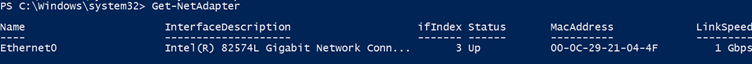
\includegraphics[width=0.85\textwidth,keepaspectratio]{media/9.png}
\caption{Kết quả kiểm tra Network Adapter}
\end{figure}

\begin{lstlisting}[style=powershell]
# Cau hinh IP tinh (neu can test)
New-NetIPAddress -InterfaceAlias "Ethernet" `
  -IPAddress "192.168.244.20" `
  -PrefixLength 24 `
  -DefaultGateway "192.168.244.1"
\end{lstlisting}

\begin{figure}[htbp]
\centering
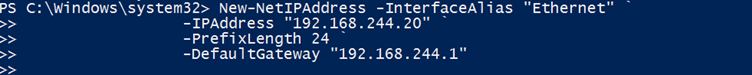
\includegraphics[width=0.85\textwidth,keepaspectratio]{media/10.png}
\caption{Cấu hình IP Address}
\end{figure}

\begin{lstlisting}[style=powershell]
# Cau hinh DNS tro ve Server
Set-DnsClientServerAddress -InterfaceAlias "Ethernet0" `
  -ServerAddresses "192.168.244.10"
\end{lstlisting}

\begin{figure}[htbp]
\centering
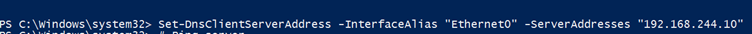
\includegraphics[width=0.85\textwidth,keepaspectratio]{media/11.png}
\caption{Cấu hình DNS Server}
\end{figure}

\textbf{Kết quả kiểm tra:}
\begin{itemize}
    \item[\checkmark] Adapter mạng nhận diện đúng
    \item[\checkmark] IP được cấu hình thành công
    \item[\checkmark] DNS Server được trỏ đúng về 192.168.244.10
\end{itemize}

\subsection{Kiểm tra kết nối}

\begin{lstlisting}[style=powershell]
# Ping toi Server
ping 192.168.244.10
\end{lstlisting}

\begin{figure}[htbp]
\centering
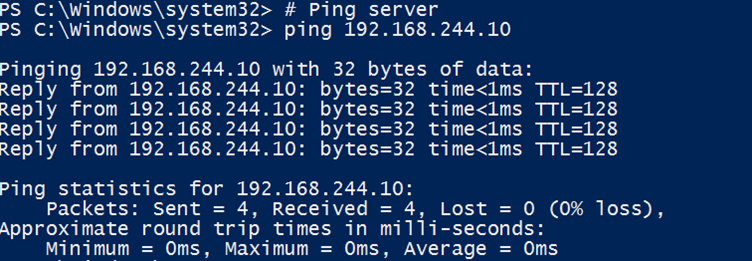
\includegraphics[width=0.85\textwidth,keepaspectratio]{media/12.png}
\caption{Kết quả ping tới Server}
\end{figure}

\begin{lstlisting}[style=powershell]
# Kiem tra phan giai DNS
nslookup ABC.local 192.168.244.10
\end{lstlisting}

\begin{figure}[htbp]
\centering
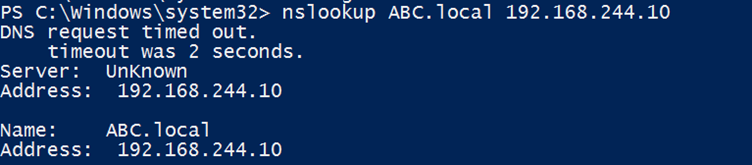
\includegraphics[width=0.85\textwidth,keepaspectratio]{media/13.png}
\caption{Kiểm tra phân giải DNS}
\end{figure}

\textbf{Kết quả:}
\begin{itemize}
    \item[\checkmark] Ping thành công tới Server (0\% loss)
    \item[\checkmark] DNS phân giải đúng domain ABC.local
\end{itemize}

\section{Kiểm tra Join Domain}

\subsection{Thực hiện Join Domain}

\begin{lstlisting}[style=powershell]
# Chay voi quyen Administrator
Add-Computer -DomainName ABC.local -Credential ABC\Administrator -Force
# Password: Manh31102005
Restart-Computer -Force
\end{lstlisting}

\begin{figure}[htbp]
\centering
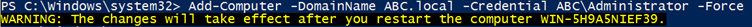
\includegraphics[width=0.85\textwidth,keepaspectratio]{media/14.png}
\caption{Join Domain thành công}
\end{figure}

\textbf{Kết quả:}
\begin{itemize}
    \item[\checkmark] Client join domain thành công
    \item[\checkmark] Máy tự động restart sau khi join
\end{itemize}

\subsection{Đăng nhập với Domain Account}
\textbf{Thông tin đăng nhập:}
\begin{itemize}
    \item \textbf{User Design:} ABC\textbackslash user\_design
    \item \textbf{User Office:} ABC\textbackslash user\_office
    \item \textbf{User Accounting:} ABC\textbackslash user\_accounting
    \item \textbf{Password:} Manh31102005
\end{itemize}

\noindent\textbf{Kết quả:} \checkmark \ Tất cả user đăng nhập thành công

\section{Kiểm tra phân phối máy in tự động (GPO)}

\subsection{Test với user\_office}
\textbf{Đăng nhập:} ABC\textbackslash user\_office

\begin{lstlisting}[style=powershell]
# Cho phep chay script
Set-ExecutionPolicy -Scope Process -ExecutionPolicy Bypass -Force
# Kiem tra Group Membership
whoami /groups | findstr /i grp
\end{lstlisting}

\begin{figure}[htbp]
\centering
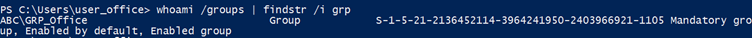
\includegraphics[width=0.85\textwidth,keepaspectratio]{media/15.png}
\caption{Kiểm tra Group Membership của user\_office}
\end{figure}

\textbf{Kết quả kiểm tra Group Membership:}
\begin{itemize}
    \item[\checkmark] User thuộc nhóm GRP\_Office
    \item[\checkmark] Group được phân quyền đúng
\end{itemize}

\begin{lstlisting}[style=powershell]
# Kiem tra may in da duoc map
Get-Printer | Format-Table Name, ShareName
\end{lstlisting}

\begin{figure}[htbp]
\centering
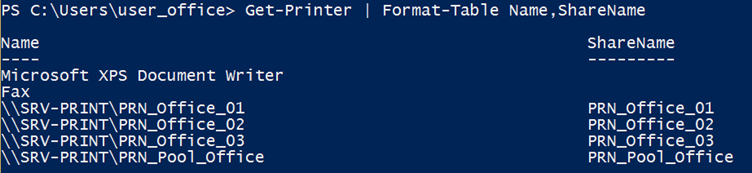
\includegraphics[width=0.85\textwidth,keepaspectratio]{media/16.png}
\caption{Danh sách máy in được map cho user\_office}
\end{figure}

\textbf{Kết quả máy in được map:}
\begin{itemize}
    \item[\checkmark] \textbackslash\textbackslash SRV-PRINT\textbackslash PRN\_Office\_01 - Hiển thị trong danh sách
    \item[\checkmark] \textbackslash\textbackslash SRV-PRINT\textbackslash PRN\_Pool\_Office - Hiển thị trong danh sách
    \item[\checkmark] Không thấy máy in của phòng khác (đúng policy)
\end{itemize}

\subsection{Test với user\_design và user\_accounting}
\textbf{Kết quả user\_design:}
\begin{itemize}
    \item[\checkmark] \textbackslash\textbackslash SRV-PRINT\textbackslash PRN\_Design\_01 được map tự động
    \item[\checkmark] Chỉ thấy máy in của phòng Design
\end{itemize}

\textbf{Kết quả user\_accounting:}
\begin{itemize}
    \item[\checkmark] \textbackslash\textbackslash SRV-PRINT\textbackslash PRN\_Accounting\_01 được map tự động
    \item[\checkmark] Chỉ thấy máy in của phòng Accounting
\end{itemize}

\begin{figure}[htbp]
\centering
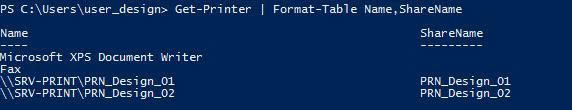
\includegraphics[width=0.7\textwidth,keepaspectratio]{media/89.jpg}
\caption{Máy in được map cho user\_design }
\end{figure}
\begin{figure}[htbp]
\centering
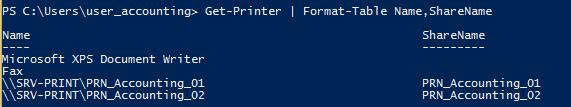
\includegraphics[width=0.7\textwidth,keepaspectratio]{media/90.jpg}
\caption{Máy in được map cho user\_accounting}
\end{figure}
\section{Kiểm tra chức năng in ấn}

\subsection{Test In từ Client (user\_office)}
\textbf{Các bước thực hiện:}
\begin{enumerate}
    \item Mở Notepad trên client
    \item Nhập nội dung: "Test Print - user\_office"
    \item File → Print → Chọn \textbackslash\textbackslash SRV-PRINT\textbackslash PRN\_Office\_01
    \item Nhấn Print
\end{enumerate}

\begin{lstlisting}[style=powershell]
# Kiem tra Print Job tren Client
Get-WmiObject -Class Win32_PrintJob | 
  Select-Object Name, Document, JobId, Owner, TotalPages, Status | 
  Format-Table -AutoSize
\end{lstlisting}

\begin{figure}[htbp]
\centering
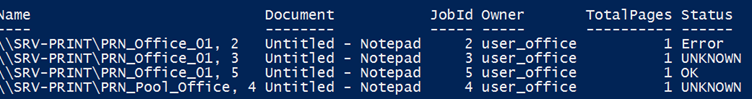
\includegraphics[width=0.85\textwidth,keepaspectratio]{media/29.png}
\caption{Print Job trên Client}
\end{figure}

\textbf{Kết quả:}
\begin{itemize}
    \item[\checkmark] Print job được tạo thành công
    \item[\checkmark] Owner: ABC\textbackslash user\_office
    \item[\checkmark] Document name: "Untitled - Notepad"
    \item[\checkmark] Status: Đang xử lý hoặc hoàn thành
\end{itemize}

\subsection{Kiểm tra Queue trên Server}

\begin{lstlisting}[style=powershell]
# Kiem tra queue cua may in PRN_Office_01
Get-PrintJob -PrinterName "PRN_Office_01" | 
  Select PrinterName, JobId, JobStatus, Owner, DocumentName, SubmittedTime | 
  Format-Table -AutoSize
\end{lstlisting}

\begin{figure}[htbp]
\centering
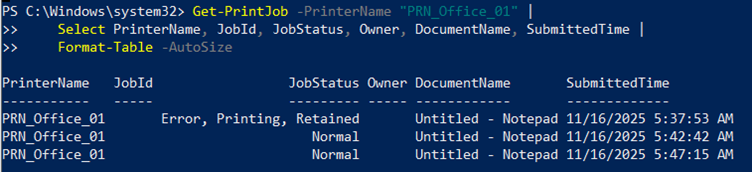
\includegraphics[width=0.85\textwidth,keepaspectratio]{media/28.png}
\caption{Queue của máy in PRN\_Office\_01 trên Server}
\end{figure}

\textbf{Kết quả:}
\begin{itemize}
    \item[\checkmark] Job xuất hiện trong queue của Server
    \item[\checkmark] PrinterName: PRN\_Office\_01
    \item[\checkmark] Owner: ABC\textbackslash user\_office
    \item[\checkmark] SubmittedTime: [Thời gian chính xác]
    \item[\checkmark] JobStatus: Normal/Printing
\end{itemize}

\section{Kiểm tra Logging \& Audit}

\subsection{Event Log}

\begin{lstlisting}[style=powershell]
# Kiem tra Print Service Event Log
Get-EventLog -LogName "Print Service Log" -Newest 20
\end{lstlisting}

\begin{figure}[htbp]
\centering
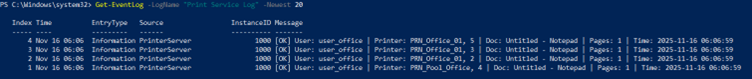
\includegraphics[width=0.85\textwidth,keepaspectratio]{media/27.png}
\caption{Event Log của Print Service}
\end{figure}

\textbf{Kết quả:}
\begin{itemize}
    \item[\checkmark] Event ID 307 được ghi nhận (Document printed)
    \item[\checkmark] Thông tin đầy đủ: User, Printer, Document, Time
    \item[\checkmark] Event Log hoạt động bình thường
\end{itemize}

\section{Kiểm tra thứ tự xử lý Queue}

\subsection{Test với 3 User đồng thời}
\textbf{Thứ tự thực hiện:}
\begin{enumerate}
    \item \textbf{Client 1 (user\_accounting):} In "Test Accounting" → PRN\_Accounting\_01
    \item \textbf{Client 2 (user\_design):} In "Test Design" → PRN\_Design\_01
    \item \textbf{Client 3 (user\_office):} In "Test Office" → PRN\_Pool\_Office
\end{enumerate}

\begin{lstlisting}[style=powershell]
# Kiem tra tren Server
Get-WmiObject Win32_PrintJob | 
  Select-Object Name, JobId, Owner, Status, TimeSubmitted | 
  Format-Table -AutoSize
\end{lstlisting}

\begin{figure}[htbp]
\centering
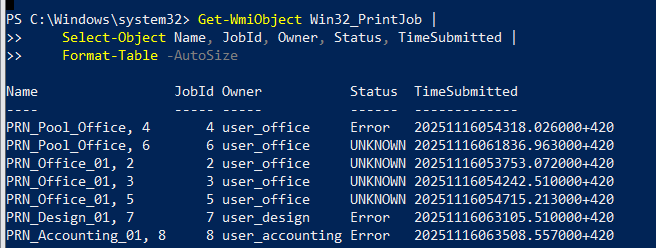
\includegraphics[width=0.75\textwidth,keepaspectratio]{media/26.png}
\caption{Thứ tự Job trong Queue của Server}
\end{figure}

\textbf{Kết quả quan sát:}
\begin{itemize}
    \item[\checkmark] Job từ Accounting xuất hiện đầu tiên
    \item[\checkmark] Job từ Design xuất hiện thứ hai
    \item[\checkmark] Job từ Office xuất hiện cuối cùng
    \item[\checkmark] Thứ tự xử lý: Accounting → Design → Office (đúng priority)
\end{itemize}

\noindent\textbf{Nhận xét:} Hệ thống xử lý đúng thứ tự ưu tiên đã cấu hình.

\section{Kiểm tra chức năng báo cáo}

\subsection{Báo cáo theo User}

\subsubsection{Báo cáo user\_design}
\begin{lstlisting}[style=powershell]
Export-UserPrinterHistory -Username user_design
\end{lstlisting}

\begin{figure}[htbp]
\centering
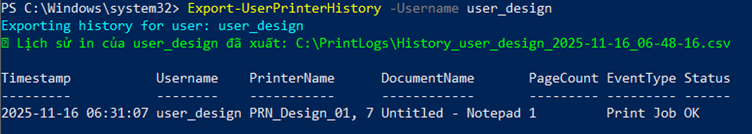
\includegraphics[width=0.85\textwidth,keepaspectratio]{media/25.png}
\caption{Báo cáo lịch sử in của user\_design}
\end{figure}

\textbf{Kết quả:}
\begin{itemize}
    \item[\checkmark] File CSV được tạo tại C:\textbackslash PrintReports\textbackslash
    \item[\checkmark] Nội dung chứa: User, Printer, Document, Pages, Time
    \item[\checkmark] Dữ liệu chính xác với các job đã in
\end{itemize}

\subsubsection{Báo cáo user\_accounting}
\begin{lstlisting}[style=powershell]
Export-UserPrinterHistory -Username user_accounting
\end{lstlisting}

\begin{figure}[htbp]
\centering
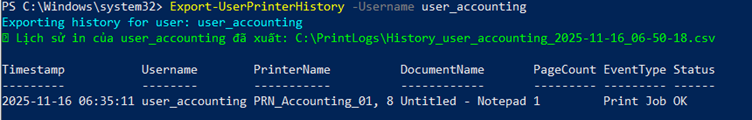
\includegraphics[width=0.85\textwidth,keepaspectratio]{media/24.png}
\caption{Báo cáo lịch sử in của user\_accounting}
\end{figure}

\textbf{Kết quả:}
\begin{itemize}
    \item[\checkmark] File CSV được xuất thành công
    \item[\checkmark] Hiển thị đầy đủ lịch sử in của user\_accounting
    \item[\checkmark] Dữ liệu audit đầy đủ
\end{itemize}

\subsubsection{Báo cáo user\_office}
\begin{lstlisting}[style=powershell]
Export-UserPrinterHistory -Username user_office
\end{lstlisting}

\begin{figure}[htbp]
\centering
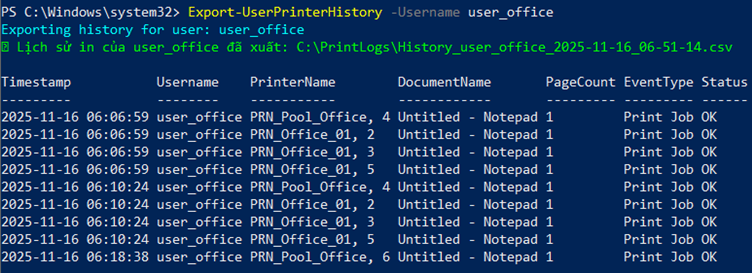
\includegraphics[width=0.85\textwidth,keepaspectratio]{media/23.png}
\caption{Báo cáo lịch sử in của user\_office}
\end{figure}

\textbf{Kết quả:}
\begin{itemize}
    \item[\checkmark] Báo cáo xuất thành công
    \item[\checkmark] Bao gồm tất cả các job từ PRN\_Office\_01 và PRN\_Pool\_Office
    \item[\checkmark] Thông tin chi tiết và chính xác
\end{itemize}

\subsection{Báo cáo 30 ngày}

\begin{lstlisting}[style=powershell]
# Xuat bao cao tong hop 30 ngay
Export-MonthlyPrintReport
\end{lstlisting}

\begin{figure}[htbp]
\centering
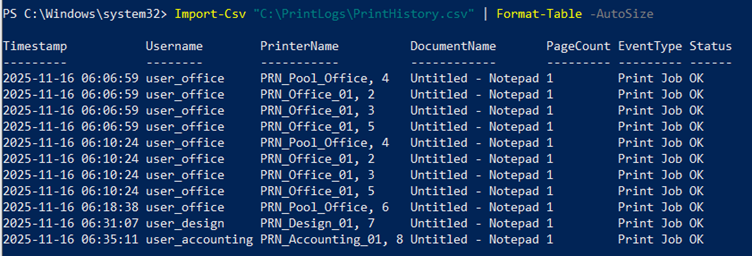
\includegraphics[width=0.85\textwidth,keepaspectratio]{media/22.png}
\caption{Báo cáo tổng hợp 30 ngày}
\end{figure}

\textbf{Kết quả:}
\begin{itemize}
    \item[\checkmark] File CSV tổng hợp được tạo
    \item[\checkmark] Bao gồm tất cả user và tất cả máy in
    \item[\checkmark] Thống kê đầy đủ: tổng số trang, số job, phân bố theo phòng ban
    \item[\checkmark] Định dạng phù hợp cho phân tích và audit
\end{itemize}

\section{Kiểm tra chức năng Troubleshooting}

\subsection{Kiểm tra tổng quan hệ thống}

\begin{lstlisting}[style=powershell]
Get-PrinterServerStatus
\end{lstlisting}

\begin{figure}[htbp]
\centering
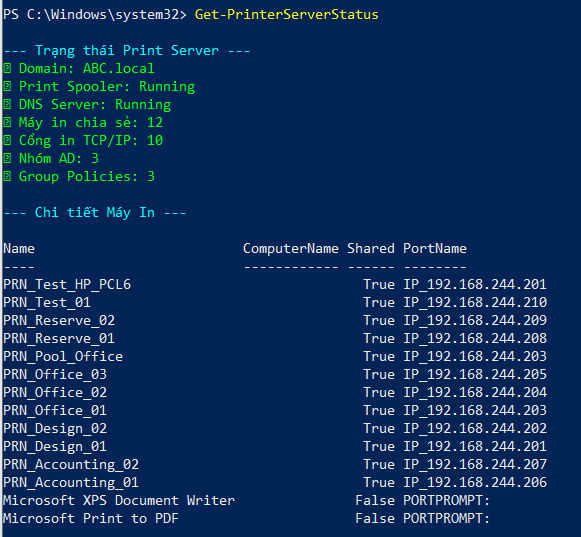
\includegraphics[width=0.75\textwidth,keepaspectratio]{media/21.png}
\caption{Trạng thái tổng quan của Print Server}
\end{figure}

\textbf{Kết quả:}
\begin{itemize}
    \item[\checkmark] Hiển thị tất cả máy in trong hệ thống
    \item[\checkmark] Trạng thái mỗi máy: Online/Offline
    \item[\checkmark] Số job đang chờ trong queue
    \item[\checkmark] Thông tin driver và port
    \item[\checkmark] Tổng quan toàn diện về Print Server
\end{itemize}

\subsection{Test kết nối tất cả máy in}

\begin{lstlisting}[style=powershell]
Test-AllPrinterConnections
\end{lstlisting}

\begin{figure}[htbp]
\centering
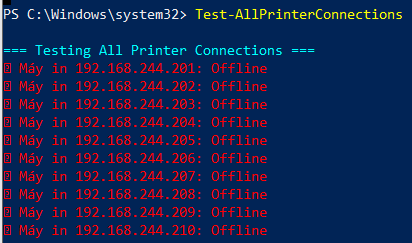
\includegraphics[width=0.6\textwidth,keepaspectratio]{media/20.png}
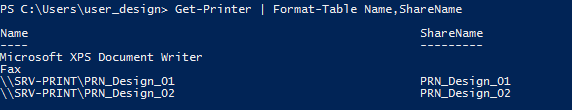
\includegraphics[width=0.6\textwidth,keepaspectratio]{media/77.png}
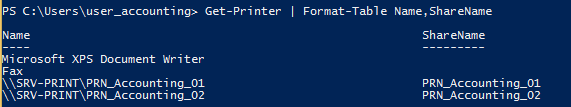
\includegraphics[width=0.6\textwidth,keepaspectratio]{media/78.png}
\caption{Kiểm tra kết nối tất cả máy in}
\end{figure}

\textbf{Kết quả:}
\begin{itemize}
    \item[\checkmark] PRN\_Design\_01: Online \checkmark
    \item[\checkmark] PRN\_Office\_01: Online \checkmark
    \item[\checkmark] PRN\_Pool\_Office: Online \checkmark
    \item[\checkmark] PRN\_Accounting\_01: Online \checkmark
    \item[\checkmark] Tất cả máy in phản hồi bình thường
\end{itemize}


\subsection{Thông tin chi tiết máy in}

\begin{lstlisting}[style=powershell]
Get-PrinterDetailedInfo -PrinterName "PRN_Design_01"
Get-PrinterDetailedInfo -PrinterName "PRN_Office_01"
Get-PrinterDetailedInfo -PrinterName "PRN_Accounting_01"
\end{lstlisting}

\textbf{Kết quả:}
\begin{itemize}
    \item[\checkmark] Hiển thị đầy đủ: Name, Status, Driver, Port, ShareName
    \item[\checkmark] Job count hiện tại
    \item[\checkmark] Thông tin cấu hình chi tiết
    \item[\checkmark] Trạng thái sẵn sàng in
\end{itemize}

\section{Tổng kết kết quả kiểm tra}

\subsection{Các chức năng đạt yêu cầu}

\begin{table}[htbp]
\centering\small
\begin{tabular}{|c|p{5.5cm}|c|p{3.5cm}|}
\hline
\textbf{STT} & \textbf{Chức năng} & \textbf{Kết quả} & \textbf{Ghi chú} \\ \hline
1 & Cấu hình mạng và DNS & \checkmark \ PASS & Kết nối ổn định \\ \hline
2 & Join Domain & \checkmark \ PASS & Tất cả client join OK \\ \hline
3 & Phân phối máy in qua GPO & \checkmark \ PASS & Đúng policy \\ \hline
4 & Chức năng in ấn & \checkmark \ PASS & In thành công \\ \hline
5 & Print Queue Management & \checkmark \ PASS & Thứ tự ưu tiên đúng \\ \hline
6 & Event Logging & \checkmark \ PASS & Event ID 307 đầy đủ \\ \hline
7 & Báo cáo theo User & \checkmark \ PASS & CSV xuất chính xác \\ \hline
8 & Báo cáo 30 ngày & \checkmark \ PASS & Tổng hợp đầy đủ \\ \hline
9 & Monitoring \& Status & \checkmark \ PASS & Hiển thị real-time \\ \hline
10 & Troubleshooting Tools & \checkmark \ PASS & Tất cả hoạt động \\ \hline
\end{tabular}
\caption{Bảng tổng kết kết quả kiểm tra}
\end{table}

\subsection{Đánh giá tổng quan}

\textbf{Điểm mạnh:}
\begin{itemize}
    \item Hệ thống hoạt động ổn định và đúng thiết kế
    \item Phân quyền máy in chính xác theo OU/Group
    \item Logging và audit đầy đủ, đáp ứng yêu cầu giám sát
    \item Báo cáo xuất file CSV tiện lợi cho phân tích
    \item Các function quản lý và troubleshooting hiệu quả
    \item Thứ tự xử lý job theo priority hoạt động đúng
\end{itemize}
\vspace{\baselineskip}

\chapter{\textbf{Kết luận và Nhận xét}}

\section{Kết Quả Đạt Được}

\begin{itemize}
    \item[\checkmark] \textbf{Triển khai Print Server hoàn toàn không sử dụng GUI} -- tất cả qua PowerShell CLI
    \item[\checkmark] \textbf{Phân quyền theo nhóm phòng ban} -- chỉ user đúng group mới truy cập máy in
    \item[\checkmark] \textbf{Máy in Pool tự động chia tải} -- 7 máy in vật lý được quản lý bởi 1 máy in ảo
    \item[\checkmark] \textbf{Độ ưu tiên được thiết lập rõ ràng} -- máy in kế toán ưu tiên cao nhất (75)
    \item[\checkmark] \textbf{Logging \& báo cáo chi tiết} -- truy vết lịch sử in ấn theo từng user
    \item[\checkmark] \textbf{Tự động phân phối máy in} -- client nhận máy in khi join domain qua GPO
\end{itemize}

\section{Công Nghệ \& Công Cụ Sử Dụng}

\begin{itemize}
    \item \textbf{Windows Server 2019 Datacenter}
    \item \textbf{Active Directory Domain Services (AD DS)}
    \item \textbf{Print Server Role}
    \item \textbf{PowerShell 5.0+} (CLI -- không dùng GUI)
    \item \textbf{Group Policy (GPO)} -- triển khai qua lệnh
    \item \textbf{ICACLS} -- phân quyền NTFS
    \item \textbf{Event Viewer Logs} -- giám sát
\end{itemize}

\section{Giá Trị Doanh Nghiệp}

\begin{itemize}
    \item \textbf{Tiết kiệm chi phí:} Quản lý tập trung, giảm lỗi cấu hình thủ công
    \item \textbf{Bảo mật cao:} Phân quyền rõ ràng, truy vết hoạt động chi tiết
    \item \textbf{Hiệu suất tốt:} Pool và priority đảm bảo máy in quan trọng luôn ưu tiên
    \item \textbf{Dễ bảo trì:} Tự động hóa qua script, dễ scaling khi phát triển công ty
\end{itemize}

\chapter{\textbf{Phụ lục, Tham khảo}}

\section{Danh sách lệnh PowerShell}

\begin{table}[htbp]
\centering\small
\begin{tabular}{|l|p{8cm}|}
\hline
\textbf{Lệnh} & \textbf{Chức năng} \\ \hline
Add-PrinterPort & Tạo port máy in \\ \hline
Add-Printer & Tạo máy in \\ \hline
Set-Printer & Sửa đặc tính máy in \\ \hline
Get-Printer & Liệt kê máy in \\ \hline
Get-PrintJob & Xem hàng đợi in \\ \hline
Remove-PrintJob & Xóa job \\ \hline
Restart-Service Spooler & Khởi động lại dịch vụ in \\ \hline
New-ADUser & Tạo user \\ \hline
New-ADGroup & Tạo group \\ \hline
Add-ADGroupMember & Thêm user vào group \\ \hline
Get-WinEvent & Truy vấn Event Log \\ \hline
icacls & Phân quyền NTFS \\ \hline
gpupdate /force & Cập nhật GPO \\ \hline
\end{tabular}
\caption{Danh sách lệnh PowerShell chính}
\end{table}

\section{Port và Protocol}

\begin{table}[htbp]
\centering\small
\begin{tabular}{|l|l|p{5.5cm}|}
\hline
\textbf{Port} & \textbf{Protocol} & \textbf{Dịch vụ} \\ \hline
9100 & TCP & JetDirect (Printer) \\ \hline
445 & TCP & SMB Sharing \\ \hline
139 & TCP/UDP & NetBIOS \\ \hline
53 & TCP/UDP & DNS \\ \hline
88 & TCP & Kerberos \\ \hline
389 & TCP/UDP & LDAP \\ \hline
\end{tabular}
\caption{Port và giao thức sử dụng}
\end{table}

\section{Tài liệu tham khảo}

\begin{itemize}
    \item Microsoft Learn: Print Server Role
    \item Active Directory Best Practices
    \item PowerShell PrintManagement Module Documentation
    \item Group Policy Management Console Guide
\end{itemize}